\section{Methods}
\label{section:methods}

Bijels require a multi-scale model to correctly simulate all the physical phenomena occurring at every scale. Within a bijel, fluid flow,
phase separation, particle-fluid and interparticle interactions are present. The lengthscales present in a bijel imply a model must be able
to resolve nanometer to micrometer resolutions and must be able to capture the hydrodynamics, non-ideal mixing and interparticle interactions present
in the system. A review of the physics in the system will be provided. 

Mass conservation is established using simple differential equation of a control volume that characterizes the mass flow through the volume. Assuming no
addition or subtraction of mass, the differential equation is the material derivative of the density, defined as

\begin{equation}
    \frac{\partial\rho}{\partial t} + \nabla\cdot\left(\rho\vec{u}\right) = 0
\end{equation}

Where $\rho$ is the fluid density and $\vec{u}$ is the fluid velocity vector. The fluid momentum can be derived from the mass conservation equation
by calculating the material derivative of the momentum of the system. Changes in momentum from addition or subtraction of momentum cannot be ignored,
with changes arising from pressure gradients, viscous forces and body force terms. If mass is conserved, the momentum equation is defined as

\begin{equation}
    \rho (\frac{\partial\vec{u}}{\partial t} + (\vec{u}\cdot\nabla)\vec{u}) = -\nabla p + \nabla \cdot \mathbf{\tau} + \mathbf{f}
\end{equation}

Where $p$ is the pressure applied to the control volume, $\mathbf{\tau}$ is a general stress tensor and $\mathbf{f}$ is the body force 
applied on the box such as gravitational forces. $\mathbf{\tau}$ can be defined by assuming the fluid is isotropic, the shear stress depends
linearly on the dynamic viscosity and the strain rate and net forces are zero at equilibrium.

\begin{equation}
    \mathbf{\tau} = p\mathbf{I} + \eta(\nabla \mathbf{v} + (\nabla \mathbf{v})^T) - \frac{2}{3}\eta(\nabla \cdot \mathbf{v})\mathbf{I}
\end{equation}

Where $p = (\lambda + \frac{2}{3}\eta)\nabla \cdot \mathbf{v}$ is defined from the bulk viscosity $\lambda$. After substitution into the momentum equation, the compressible 
Navier Stokes equation is obtained, defined as

\begin{equation}
    \rho (\frac{\partial\vec{u}}{\partial t} + (\vec{u}\cdot\nabla)\vec{u}) = -\nabla p + \eta \Delta \mathbf{v} + \frac{1}{3}\eta \nabla(\nabla \cdot \mathbf{v}) + \mathbf{f}
\end{equation}

If the fluid being modelled is assumed to be incompressible meaning that the density stays constant and the bulk viscosity is 0, $\nabla \cdot \mathbf{v} = 0$. This simplifies
the Navier Stokes equation to

\begin{equation}
    \rho (\frac{\partial\vec{u}}{\partial t} + (\vec{u}\cdot\nabla)\vec{u}) = -\nabla p + \eta \Delta \mathbf{v} + \mathbf{f}
\end{equation}

The Navier Stokes equation can be recast into a dimensionless form by rescaling length, time and density into dimensionless forms. These parameters are rescaled as 
$\bar{l} = \frac{l}{l_0}$, $\bar{t} = \frac{t}{t_0}$ and $\bar{\rho} = \frac{\rho}{\rho_0}$ with barred quantities indicating dimensionless properties. After substituting
these parameters into the Naver Stokes equation this is obtained

\begin{equation}
    \frac{\partial \bar{\vec{u}}}{\partial \bar{t}} + (\bar{\vec{u}} \cdot\nabla)\bar{\vec{u}} = -\nabla \bar{p} + \frac{1}{Re} \Delta \mathbf{\bar{v}} + \bar{\mathbf{f}}
\end{equation}

$Re = \frac{\rho u l}{\eta}$ which defines the ratio between inertial and viscous forces. Another physical phenomenon being described is non-ideal mixing. The free energy of mixing
is defined as $\Delta G_m = \Delta H_m - T \Delta S_m$. In an ideal solution, $\Delta H_m = 0$. An expression for $\Delta S_m$ for a binary mixture is obtained from statistical mechanical 
approximations of the configurations that binary mixtures can take, resulting in 

\begin{equation}
    S_m = -k N_\phi k_B T((1 - \phi)\ln{1 - \phi} + \phi ln(\phi)) 
\end{equation}

In a regular solution, $\Delta H_m \neq 0$. The free energy of mixing is defined as the sum of the ideal and excess contribution, $\Delta G_m = \Delta G_e + \Delta G_i$.
$\Delta G_i = -TS_m$. $\Delta G_e = \Delta H_e + T \Delta S_e$. The excess entropy of mixing is 0, and the excess enthalpy of mixing is defined 

The Shan-Chen pseudopotential
model is used to simulate the Cahn-Hilliard equation, defined below

\begin{equation}
    \begin{split}
    \frac{\partial\phi}{\partial t}+\nabla\cdot\left(\phi\vec{u}\right) &= \nabla \cdot \left( \Gamma  \nabla\phi \right)
    \end{split}
\end{equation}

where $c^k$, $M^k$ and $u^k$ is the concentration, mobility and velocity of species $k$ respectively while $\mu$ is the free energy of system. 
\cite{shan_lattice_1993, shan_simulation_1994, he_lattice_1997, he_discrete_1998}



A computational model designed to simulate soft matter systems 
at the mesoscale must accurately represent both hydrodynamics and non-ideal mixing in order to capture the essential physics of emulsions, colloids, and phase-separating fluids. 
A hydrodynamic model must be able to recover mass and momentum conservation of a incompressible fluid

Modelling multicomponent dynamics requires incorporating a free energy model between fluids, allowing for the implementation of
chemical potential driven mass transfer and surface tension. Typically this is done using a Cahn-Hilliard model based on a
square gradient free energy functional. This captures the demixing characteristics of phase separating fluids and controls interface
characteristics, providing surface tension and interface width characteristics. This model has been used in past investigations looking 
into spinodal decomposition, domain growth and coarsening. 


To fully capture mesoscale dynamics, the model must also resolve the coupling between hydrodynamic flow and composition gradients. This coupling 
is essential for simulating phenomena such as Marangoni flows, interfacial instabilities, and anisotropic stress distributions that arise from 
non-uniform compositions or curvature-dependent surface tension. Moreover, the model must support anisotropic or time-dependent external fields 
(e.g., magnetic, electric, or shear) that influence mixing behavior. Computational frameworks that can evolve velocity, pressure, and composition 
fields simultaneously—while ensuring thermodynamic consistency and mechanical stability—are critical for accurately describing the emergent structures 
and transport properties in non-ideal soft matter systems.

Given the multiscale modeling necessary to correctly simulate the physical system, one approach suggested to tackle this problem is the multicomponent
Lattice Boltzmann Method. This technique bridges the length and time scales necessary in soft matter modeling through modeling the evolution of a particle
distribution function. Hydrodynamic parameters are recovered through calculating the moments of the particle distribution function. One of the advantages of
the Lattice Boltzmann Method its parallelize nature and ease of adding multiple physical phenomena. In the following sections, the implementation of the LBM
and alternatives to the LBM will be presented.

% This work uses a multicomponent Lattice Boltzmann Method (LBM) to simulate the hydrodynamics of two partially miscible, 
% incompressible fluids as implemented in LB3D. The LBM solves the continuity and Navier-Stokes equation at low
% Mach and Reynolds numbers for the fluid, defined as, 

% \begin{equation}
%     \begin{split}
%     \frac{\partial\rho}{\partial t} + \nabla\cdot\left(\rho\vec{u}\right) &= 0 , \\
%     \frac{\partial\vec{u}}{\partial t} + (\vec{u}\cdot\nabla)\vec{u} &= - \frac{1}{\rho} \nabla p + \nu \nabla^2 \vec{u} ,
%     \end{split}
% \end{equation}

% incorporating density $(\rho)$, viscosity $(\eta)$, velocity $(u)$, pressure $(P)$, and 
% body force $(F_{body})$. \cite{qian_lattice_1992, chin_lattice_2002, nourgaliev_lattice_2003} The Shan-Chen pseudopotential
% model is used to simulate the Cahn-Hilliard equation, defined below

% \begin{equation}
%     \begin{split}
%     \frac{\partial\phi}{\partial t}+\nabla\cdot\left(\phi\vec{u}\right) &= \nabla \cdot \left( \Gamma  \nabla\phi \right)
%     \end{split}
% \end{equation}

% where $c^k$, $M^k$ and $u^k$ is the concentration, mobility and velocity of species $k$ respectively while $\mu$ is the free energy of system. 
% \cite{shan_lattice_1993, shan_simulation_1994, he_lattice_1997, he_discrete_1998}

% Particle dynamics include Hertzian contact and lubrication forces, tracked with classical Newtonian mechanics, while 
% particle-fluid coupling involves momentum exchange to simulate viscous dissipation. Particle-particle magnetic interactions are modeled using dipole 
% interactions. \cite{davies_interface_2014, xie_direct_2017, xie_controllable_2021} A more detailed description of the model is 
% provided in the following sections

\section{Lattice Boltzmann Method}

The Lattice Boltzmann Method (LBM) is an evolution of preceding lattice gas automata techniques, which is a discretization of the Boltzmann equation of motion for 
molecules. This means that unlike traditional CFD techniques such as FDM, VOF or level set methods, LBM tracks the evolution of a 
particle distribution function within grid cells evolved through a discretized Boltzmann equation of motion. Macroscopic variables such as fluid density and 
velocity are recovered from the particle distributions through appropriate moment integration, and the Navier Stokes equation at the incompressible limit can be 
obtained through a Chapman-Enskog expansion of the LBM. The LBM has become an attractive tool for meso-scale CFD simulations due to its ease of algorithm 
implementation, highly parallelizable nature and ease of boundary condition implementation, allowing coupling to other physically relevant systems such as 
particles with varieties of potentials, external fields and deformable bodies.

The particle distribution function described earlier is advected on a pre-constructed lattice stencil, commonly denoted as DnQm where n and m represent the 
number of dimensions and directions in the stencil. Common stencils include the D1Q5, D2Q9 and D3Q19 stencil, all of which recover mass and momentum conservation. 
For energy conservation, a higher order stencil such as D3Q27 is necessary. The D2Q9 and D3Q19 stencils have 8 and 18 populations respectively that include 
connections to nearest and next nearest neighbour points, in addition to a central rest point. The D3Q19 stencil is shown in Figure \ref{fig:d3q19_lattice}.

\begin{figure}[h]
    \centering
    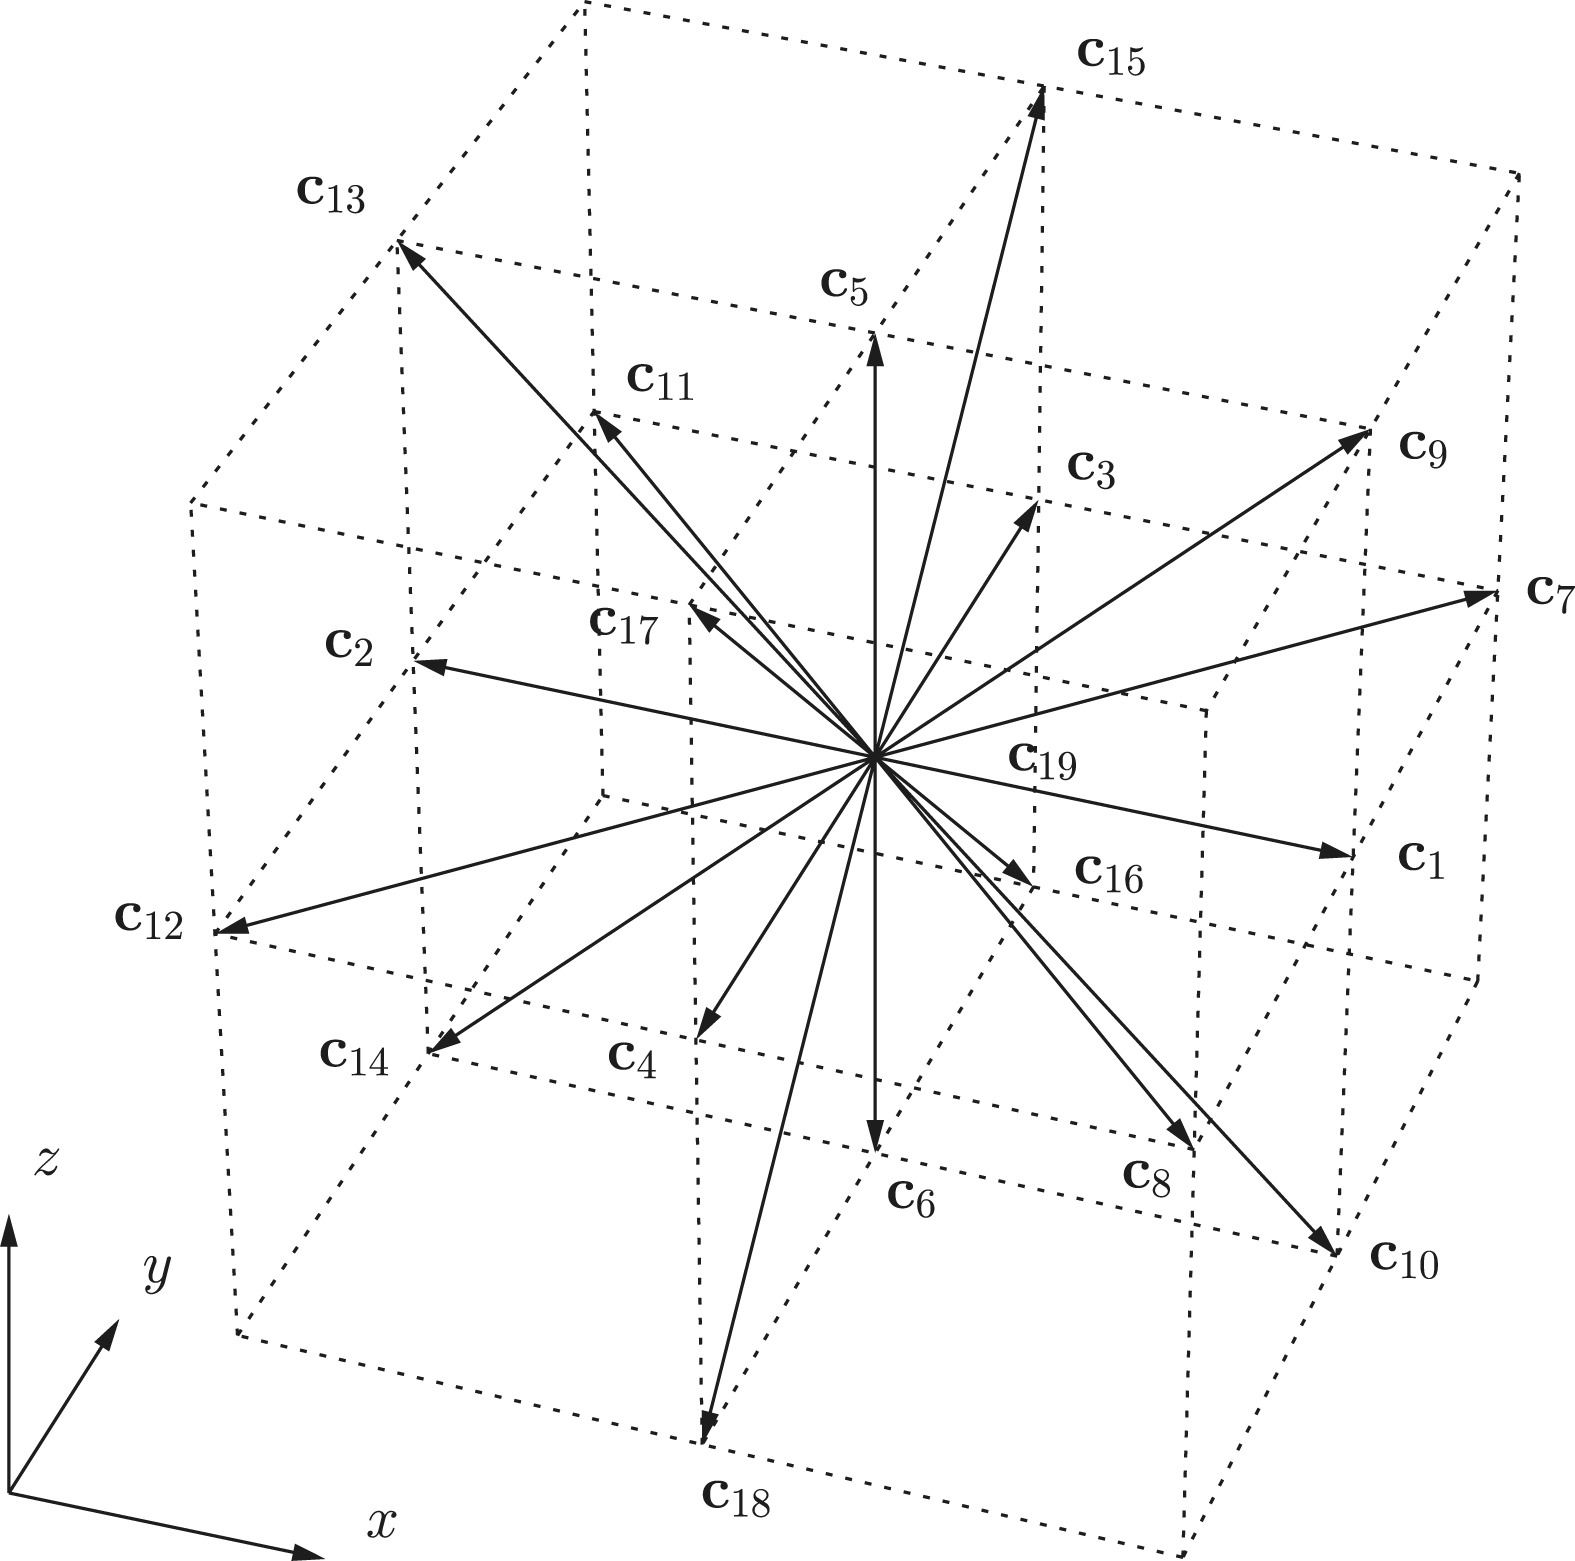
\includegraphics[scale = 1]{figures/methods/d3q19_lattice.jpg}
    \caption{D3Q19 lattice demonstrating the rest, nearest and next nearest direction that correspond to the 19 
    directions $(i)$ of the lattice with lattice velocity $c_{i}$. \cite{schmieschek_lb3d_2017} Reproduced from 
    Schmieschek et al. Computer Physics Communications 2017, 217, 149--161, under the Creative Commons license.}
    \label{fig:d3q19_lattice}
\end{figure}

The LBM is composed of a collision and advection step. In the advection step, the populations at each grid point are propagated to adjacent points in accordance 
with the chosen stencil. During the collision step, the particle population distribution is relaxed towards an equilibrium with a collision operator, at a 
specified relaxation rate. 

\section{Hydrodynamics} 
\label{section:lbm_hydrodynamics}

The lattice boltzmann method works by evolving a population distribution $f_{i}(\mathbf{x}, t)$ on a cubic lattice with 
timestep $\Delta t$ with lengthscale $\Delta x$. \cite{qian_lattice_1992, succi_lattice_2018, he_theory_1997} The D3Q19 
velocity set is used in this work with the indexes $i$ represent each of the 19 velocities and conserves mass and momentum 
to the second order. It can be seen in Figure \ref{fig:d3q19_lattice}. The algorithm is split into the 
collision step where the populations on each lattice grid cell is relaxed towards an equilibrium, followed by the 
advection step where populations in each velocity direction are propagated with velocity $\mathbf{c_i}$. 

% The collision step occurs using a single relaxation time Bhatnagar-Gross-Krook (BGK) collision operator at relaxation 
% rate $\tau$. \cite{bhatnagar_model_1954, qian_lattice_1992} 

% The collision operator can have multiple forms based on how many relaxation rates are used although the most common variant is the 
% Single Relaxation Time (SRT) collision operator, more commonly known as the Bhatnagar-Gross-Krook (BGK) collision operator. 
% \cite{bhatnagar_model_1954, qian_lattice_1992} 
% Owing to its stability in low Mach 
% and Reynolds numbers and simplicity of implementation, the BGK operator is often used in particle laden flow and soft matter simulations. 
% \cite{bhatnagar_model_1954} These limitations are present owing to the implicit link between the fluid properties and the relaxation rate, 
% and to ensure fluid incompressibility from an equation that intrinsically simulates a compressible fluid. To get over these 
% limitations, Two Relaxation Time (TRT) and Multiple Relaxation Time (MRT) operators also exist, expanding the possible application of the LBM to visco-elastic 
% flows and implementation of fluctuating hydrodynamics in the LBM. \cite{liu_simulation_2023, adhikari_fluctuating_2005} The combined collision and advection 
% LBM is expressed below in equation \ref{eq:LBM_BGK}

The collision step in the LBM is performed using the collision operator. It can take multiple forms depending on the number of
relaxation rates used. The most commonly used variant is the Single Relaxation Time (SRT) operator defined with the Bhatnagar-Gross-Krook (BGK) 
collision operator \cite{bhatnagar_model_1954, qian_lattice_1992}. The BGK model is easy to implement and works well enough in soft matter and
particle-laden flow simulations.

However the BGK operator controls all moments at a single relaxation rate which can induce numerical instabilities and inaccuracies
at higher fluid velocities. \cite{liu_simulation_2023, adhikari_fluctuating_2005} These numerical instabilities can be resolved by using
a Multiple Relaxation Time (MRT) collision operator. However the relaxation rates used in an MRT collision operator must be tuned carefully
to ensure that the appropriate fluid properties are modelled. Simpler variants of the MRT collision operator such as the Two Relaxation Time (TRT)
collision operator have been proposed as a solution that provides some of the benefits of MRT models with the simplicity of SRT models. These 
have facilitated simulation of a wider range of physical phenomena \cite{adhikari_fluctuating_2005, liu_simulation_2023}. The SRT collision 
operator is selected due to the additional computational performance needed by MRT not being needed. The combined streaming and 
collision step in LBM, using the BGK operator, is expressed in Equation \ref{eq:LBM_BGK}.

\begin{equation}
    f_{i}(\mathbf{x} + \mathbf{c}_{i}\Delta t, t + \Delta t) = f_{i}(\mathbf{x}, t) - \frac{1}{\tau}(f_{i}(\mathbf{x}, t) 
    - f_{i}^{eq}(\mathbf{x}, t))
    \label{eq:LBM_BGK}
\end{equation}

The BGK operator limits simulations to low reynolds number and mach numbers to prevent numerical instabilities. 
\cite{qian_lattice_1992} The kinematic viscosity if using the BGK operator is defined as 
$\nu = c_s^2(\tau - \frac{\Delta t}{2})$. The equilibrium distribution is obtained from a taylor expansion of the 
Maxwell-Boltzmann distribution to the second order. \cite{he_theory_1997, succi_lattice_2018} This is shown in equation 
\ref{eq:LBM_Feq}.

\begin{equation}
    f_{i}^{eq}(\mathbf{x}, t) = w_i\rho(1 + \frac{\mathbf{c_i} \cdot \mathbf{u}}{c_s^2} + \frac{(\mathbf{c_i} \cdot 
    \mathbf{u})^2}{2c_s^4} + \frac{\mathbf{u} \cdot \mathbf{u}}{2c_s^2})
    \label{eq:LBM_Feq}
\end{equation}

$\rho$ and $\textbf{u}$ in Equation \ref{eq:LBM_Feq} are defined as the macroscopic parameters for density and velocity 
and can be calculated from the mass distribution using $\rho = \sum f_i$ and $\rho \mathbf{u} = \sum f_i \mathbf{c}_i$ 
respectively. Using the Chapman-Enskog expansion, the Navier-Stokes equation at the incompressible limit at low mach
numbers can be recovered. \cite{qian_lattice_1992, he_lattice_1997} The regime accessible through this method is suitable 
for simulations in this work as the $ 1 \leq Re \leq 100 $ and the mach number, $Ma < 0.01$, fulfilling the stability 
criterion and usage requirements for the presented hydrodynamic model.

\section{Non-ideal mixing}
\label{section:lbm_non_ideal_mixing}

Four primary techniques to model multicomponent or multiphase systems exist in the LBM literature. They are the Shan-Chen (SC) pseudopotential
model, the free energy (FE) model, the color gradient (CG) model and the interface tracking (IT) model. All techniques are fundamentally different to one
another in implementation and tradeoff various properties. Each one will be briefly reviewed before a comparing and contrasting their applicability
to this system. 

The SC model introduces fluid interactions via a density-dependent force, enabling spontaneous phase separation 
and interface formation without explicitly tracking the interface. It is simple to implement and computationally efficient. However the density
dependence of the fluid interactions implies that the surface tension is controlled by the density of the fluids used and the strength parameter
controlling interactions.

The FE model derives from the implementation of a modified equilibrium distribution derived from a square gradient free energy functional. Similar to the
SC model, the FE model enables spontaneous phase separation and interface formation without explicitly tracking the interface. The surface tension and
interface width are explicitly defined from the bulk free energy, allowing for user defined surface tensions and interface widths. However in its multicomponent
implementation, it cannot be used to simulate fluids with high density ratios.

The CG model is defined with fluid components with color labels, followed by the application of a recoloring step to sharpen the interface. 
\cite{liu_multiphase_2016} The recoloring step creates the surface tension present in phase separated multicomponent mixtures. This model
provides fine control over the surface tension and narrow interface widths. However implementing the recoloring step is computationally complex 
and requires tuning of the recoloring step to ensure numerical consistency.  
% technique proposed by Latva-Kokko and Rothman is more commonly used for soft matter flows. \cite{liu_multiphase_2016}

The IT model is defined using a level-set or front-tracking techniques coupled to LBM. This technique explicitly tracks the location of the
interface by evolving a separate interface indicator. It offers the highest accuracy at capturing the interface. However it is computationally
expensive and less suited to topological changes like coalescence. 

% A quick review of the Shan-Chen (SC) or 
% pseudopotential model will be provided here from the perspective of a binary mixture. Additionally, the names and descriptions of 
% other techniques will be described as well. The interparticle potential model or Shan-Chen model that adds a non-local density dependent force 
% between two species, effectively modelling non-ideal mixing and recovering the Cahn-Hilliard equation. To alleviate the standard Shan-Chen implementations 
% weaknesses of not being thermodynamically consistent and reducing the existence of spurious velocities, thermodynamically consistent equations of state
% such as the Van der walls or Carnahan Starling equations of state have been implemented and compared to the Shan-Chen equation of state. 

% In addition to the Shan-Chen model, the color gradient model, free energy model and interface tracking technique all 
% allow for simulations of various types of multiphase and/or multicomponent flows. The color gradient model proposed by Rothman and Keller and 
% implemented by Gunstensen et al relies upon modelling two particle distributions. These represent a binary fluid mixture with the collision step 
% able to recover the hydrodynamics and non-ideal mixing dynamics. The free energy model utilizes phase field theory and constructs a free energy 
% functional to recover interfacial dynamics and effects in a thermodynamically consistent manner. Often, a square gradient free energy is used for 
% simplicity and ease of implementation. The mean field theory The non-ideal mixing dynamics are 6

Compared to other multicomponent methods, the SC model provides the 

The SC model mimics Cahn-Hilliard type behaviour through a force applied from the other fluid species $k'$ in adjacent 
cells $\mathbf{x'}$ on fluid species $k$ at point $\mathbf{x}$. \cite{shan_lattice_1993, shan_simulation_1994, 
shan_multicomponent_1995, he_discrete_1998, jansen_bijels_2011, chin_lattice_2002} Both fluid species are defined
by their own distribution equation defined in Equation \ref{eq:LBM_BGK} The strength of this force is controlled 
through an interaction parameter, $g_{kk'}$ with no contribution from self interaction of the fluid as these are 
set to zero. The SC force can then be written out in Equation \ref{eq:sc_model}.

\begin{equation}
% F_{k}^{SC}(\mathbf{x}, t) = -\Psi^{k}(\mathbf{x}, t)\sum_{k'}g_{cc'}\sum_{\mathbf{x'}}\Psi_{k'}(\mathbf{x'}, t)(\mathbf{x'} 
% - \mathbf{x})
\vec{F}_k(\vec{x}) \Delta t = - \sum_{k'} \sum_i \frac{w_i}{c_s^2} g_{kk'} \psi_k(\vec{x})\psi_{k'}(\vec{x}+\vec{c}_i) \vec{c}_i
\label{eq:sc_model}
\end{equation}

An effective mass of each fluid at node $\mathbf{x}$ is used in place of the actual density to scale it between zero 
and one and is defined as $\psi^{k}(\mathbf{x},t) = \rho_{0}\left[1 - \exp(-\frac{\rho^{k}(\mathbf{x}, t)}{\rho_{0}})\right]$. 
In this model, the SC force is incorporated into the macroscopic velocities that are then used to calculate the equilibrium
distribution $f_{i}^{k, eq}$ for fluid $k$, defined as,

\begin{equation}
\vec{u}_k^{\text{eq}} = \vec{u}' + \frac{\tau_k}{\rho_k} \vec{F}_k
\end{equation}

Where $\vec{u}'$ is defined as the common grid velocity and is calculated from $f_i^k$ below

\begin{equation}
    \sum_k \frac{\rho_k}{\tau_k} \vec{u}' = \sum_k \frac{1}{\tau_k}\sum_i f_i^k\vec{c}_i
\end{equation}

This recasting of the velocity ensures that in the absence of forces, the total momentum of the system is conserved. 

% \textcolor{blue}{https://doi.org/10.1103/PhysRevE.84.046710}

\section{Suspended particle dynamics}
\label{section:lbm_colloids}

Suspended particles will be coupled to the LB fluid based on the work conducted by Ladd. \cite{ladd_numerical_1994, 
aidun_direct_1998, ladd_lattice-boltzmann_2001} The particles follow Newtonian mechanics with the particle force and
rotational inertia defined using differential equations

\begin{equation}
    \begin{split}
    \vec{F_p} = m_p \frac{\vec{u}_p}{dt} , \\
    \vec{D_p} = \mathbf{J}_p \frac{\vec{\omega}_p}{dt} ,
    \label{eq:md}
    \end{split}
\end{equation}

$\mathbf{F_p}$ and $\mathbf{D_p}$ represent the force and torque acting on a particle with mass $m_p$ and moment of inertia 
$\mathbf{J}_p$. $\mathbf{u}_p$ and $\mathbf{\omega_{p}}$ are the linear and angular velocities of the particle. The equations of 
motion are evolved over time using a leapfrog integrator. \cite{jansen_bijels_2011}

The particles are discretized on the lattice according to the method laid out in Ladd and Aidun 
\cite{ladd_lattice-boltzmann_2001}. Nodes representing the particle are marked as solid nodes that replicate
a no-slip boundary condition through a moving bounce-back boundary. This is implemented into the distribution function
by reflecting the outgoing populations of $f_i^k$ to the opposite lattice velocity

\begin{equation}
    f^k_{i^\star}(\vec{x}, t+\Delta t) = f^{k,\star}_i(\vec{x}, t) - \frac{2w_i}{c_s^2} \rho \vec{u}_i \cdot \vec{c}_i ,
\end{equation}

This facilitates momentum exchange between particle and fluid which can be calculated analytically as 
\(\Delta\vec{p}^k_i \frac{\Delta t}{(\Delta x)^3} = 2 f^{k,\star}_i(\vec{x},t)\vec{c}_i - \frac{2w_i}{c_s^2}\rho(\vec{u}_i\cdot\vec{c}_i)\vec{c}_i\).
The sum of the momentum change across the surface of the particle is computed to obtain the force and torque on the particle,

\begin{equation}
    \begin{split}
    \vec{F}_p &= \sum_{k,i} \frac{\Delta \vec{p}^k_i}{\Delta t} , \\
    \vec{T}_p &= \sum_{k,i} \frac{\Delta\vec{p}^k_i}{\Delta t} \times \vec{r}_i .
    \end{split}
\end{equation}

As the particle moves, the nodes representing the particle are updated, with newly covered grid points marked as solid and 
uncovered nodes marked as fluid. When a grid point is covered, the momentum contained in that lattice point is added to the 
total force of the particle,

\begin{equation}
    \vec{F}_p = -\sum_{k,i} f_i^k(\vec{x},t)\vec{c}_i .
\end{equation}

Upon uncovering of a grid point, it is assigned a density value that represents the average of all adjacent fluid sites,

\begin{equation}
    \rho^k(\vec{x},t) = \frac{1}{N_{\text{f}}} \sum_{i_{\text{f}}} \rho^k(\vec{x}+\vec{c}_{i_{\text{f}}n}, t)
    \label{eq:fill_particles}
\end{equation}

\subsection{Anisotropic particles}
\label{section:lbm_colloids_ellipsoids}

For particles close to contact, meaning with inter-surface distances under 1 lattice unit the hydrodynamics are unresolved as the
distance is smaller than what the model can resolve. Lubrication forces are added to reduce the likelihood of particle overlap. For 
spherical particles, this is defined in Equation \eqref{eq:lubrication}

\begin{equation}
    \vec{F}_l = -6 \pi \eta \frac{R_1^2 R_2^2}{\left(R_1+R_2\right)^2}\left(\frac{1}{|\vec{r}_{ij}|-R_1-R_2}-\frac{1}{d_c}\right) \frac{\left(\vec{u}_{12}\cdot\vec{r}_{12}\right)\vec{r}_{12}}{|\vec{r}_{12}|^2} ,% \qquad d<d_c,
    \label{eq:lubrication}
\end{equation}

where $R_i$ and $R_j$ are the radii of each particle involved in the interaction, $\vec{r}_{ij}$ is the distance
vector between the particle centers, $\mathbf{u}_{ij}$ are the relative velocities of the particles and $\Delta_c$ 
is the cutoff distance when the lubrication force begins to act. If particles are able to overcome the lubrication forces, 
a hertzian contact force is also added to ensure that there is no particle overlap, defined in Equation \eqref{eq:hertz}

\begin{equation}
    \phi_{H} = K_{H}(R_i + R_j - |\mathbf{r}_{ij}|)^{5/2}, r < R_i + R_j
    \label{eq:hertz}
\end{equation}

$K_H$ is the force constant used to push particles apart. To correct for the anisotropic particles used in this work, 
the formulas presented in Eqs \ref{eq:lubrication} and \ref{eq:hertz} can be generalized using the route followed 
in Gunther et al. and Davies et al., inspired by Berne and Pechukas. \cite{gunther_timescales_2014, davies_interface_2014} 
They first begin by rewriting the lubrication and Hertzian contact forces as a function of the particle orientation and 
aspect ratio of the particles.

\begin{equation}
    \begin{split}
    \phi(\vec{r}_{ij}) &= {\epsilon} \tilde{\phi}\left(\frac{\vec{r}_{ij}}{{\sigma}}\right) , \\
    \vec{F}(\vec{r}_{ij}) &= {\epsilon} \tilde{\vec{F}}\left(\frac{\vec{r}_{ij}}{{\sigma}}\right) .
    \end{split}
\end{equation}

For the lubrication force \eqref{eq:lubrication}, we choose
${\sigma}=R_1+R_2$ and ${\epsilon}=\frac{6\pi\eta R_1^2 R_2^2}{{\sigma^3}}$, and for the
Hertz potential we chose ${\sigma}=R_1+R_2$ and ${\epsilon}=K_H\sigma^{5/2}$. For two identical, rotationally
symmetric ellipsoidal particles with orientations $\hat{\vec{o}}_i$ and $\hat{\vec{o}}_j$, we then replace $\epsilon$ and $\sigma$ by
the anisotropic functions

\begin{equation}
    \begin{split}
    \tilde\epsilon\left(\hat{\vec{o}}_i, \hat{\vec{o}}_j\right) &= \frac{{\epsilon}}{\sqrt{1-\chi^2}} , \\
    %\qquad \chi = \frac{\left(\alpha^2-1\right)R_\parallel^2}{\left(\alpha^2+1\right)R_\parallel^2}\left(\hat{\vec{o}}_i\hat{\vec{o}}_j\right) , \\
    \tilde\sigma\left(\vec{r}_{ij}, \hat{\vec{o}}_i, \hat{\vec{o}}_j\right) &= \frac{{\sigma}}{\sqrt{1-\frac{\chi}{2}\left[ \frac{\left(\hat{\vec{r}}_{ij}\cdot\hat{\vec{o}}_i+\hat{\vec{r}}_{ij}\cdot\hat{\vec{o}}_j\right)^2}{1+\chi\left(\hat{\vec{o}}_i\hat{\vec{o}}_j\right)} + \frac{\left(\hat{\vec{r}}_{ij}\cdot\hat{\vec{o}}_i-\hat{\vec{r}}_{ij}\cdot\hat{\vec{o}}_j\right)^2}{1-\chi\left(\hat{\vec{o}}_i\hat{\vec{o}}_j\right)} \right] }} , \\
    \chi &= \frac{\alpha^2-1}{\alpha^2+1} , \\
    \end{split}
\end{equation}

where $R_{\parallel}$ is the particle radius along the
symmetry axis $\hat{o}$ and $\alpha=\frac{R_{\parallel}}{R_{\perp}}$ the aspect
ratio of the particle. The anisotropic Hertz potential and lubrication
force are then defined as
%
\begin{equation}
    \begin{split}
    \phi\left(\vec{r}_{ij}, \hat{\vec{o}}_i, \hat{\vec{o}}_j\right) &= \epsilon\left(\hat{\vec{o}}_i, \hat{\vec{o}}_j\right) \tilde{\phi}\left(\frac{\vec{r}_{ij}}{\sigma\left(\vec{r}_{ij}, \hat{\vec{o}}_i, \hat{\vec{o}}_j\right)} \right) , \\
    \vec{F}\left(\vec{r}_{ij}, \hat{\vec{o}}_i, \hat{\vec{o}}_j\right) &= \epsilon\left(\hat{\vec{o}}_i, \hat{\vec{o}}_j\right) \tilde{\vec{F}}\left(\frac{\vec{r}_{ij}}{\sigma\left(\vec{r}_{ij}, \hat{\vec{o}}_i, \hat{\vec{o}}_j\right)} \right) .
    \end{split}
\end{equation}

\subsection{Magnetic field and particle coupling}
\label{section:lbm_colloids_magnetics}

The magnetic dipole potential is defined as

\begin{equation}
    \mathbf{U_{ij}} = \frac{\mu_0 m_i m_j}{4\pi r_{ij}^{3}} \left[ \Hat{\mathbf{o_i}} \cdot \Hat{\mathbf{o_j}} - 
    3(\Hat{\mathbf{o_i}} \cdot \Hat{\mathbf{r_{ij}}})(\Hat{\mathbf{o_j}} \cdot \Hat{\mathbf{r_{ij}}}) \right]
    \label{eq:magnet_potential}
\end{equation}

Where $\mu_0 = 4\pi \cdot 10^{-7} \frac{H}{m}$,  $\Hat{\mathbf{o_i}}$ is the orientation unit vector of particle 
$i$, $\Hat{\mathbf{r_{ij}}}$ is the distance vector between particles $i$ and $j$ and $m_i$ is the magnitude the 
magnetic dipole of particle $i$. From the potential, the force and torque of the dipole force between particles 
can be found. These expressions are shown in equations \ref{eq:dipole_magnetic_force} and \ref{eq:dipole_magnetic_torque} 
for the force and torque respectively.

\begin{equation}
    \mathbf{F}_{ij} = \frac{3 \mu_0}{4 \pi} [\frac{5(m_i \cdot \mathbf{r}_{ij})(m_j 
    \cdot \mathbf{r}_{ij})}{|\mathbf{r}_{ij}|^7}\mathbf{r}_{ij} - \frac{(m_i \cdot m_{j})\mathbf{r}_{ij} + 
    (m_i \cdot \mathbf{r}_{ij})m_i + (m_j \cdot \mathbf{r}_{ij})m_j }{|\mathbf{r}_{ij}|^5}]
\label{eq:dipole_magnetic_force}
\end{equation}

\begin{equation}
    \mathbf{T}_{ij} = \frac{\mu_0}{4 \pi}[ \frac{3(m_j \cdot \mathbf{r}_{ij})m_i \times \mathbf{r}_{ij} }
    {|\mathbf{r}_{ij}|^5} - \frac{m_i \cdot m_j }{|\mathbf{r}_{ij}|^3} ]
    \label{eq:dipole_magnetic_torque}
\end{equation}

Equations \ref{eq:magnet_force} and \ref{eq:magnet_torque} are used to calculate the force and torque that the 
field exerts on each particle.

\begin{equation}
    \mathbf{F_{j}} = (m_j \Hat{\mathbf{o_j}} \cdot \nabla B_i)
    \label{eq:magnet_force}
\end{equation}

\begin{equation}
    \mathbf{\tau_j} = (m_j \Hat{\mathbf{o_j}} \times B_i)
    \label{eq:magnet_torque}
\end{equation}

The total force and torque exerted on each particle is the sum of the particle dipole interaction and the field 
dependent contribution. 